\documentclass[12pt]{article}
\usepackage[top=1in, bottom=1in, left=1in, right=1in]{geometry}
\usepackage{graphicx}
\usepackage[colorlinks, linkcolor=black]{hyperref}

\title{One Minute Tutorial of CurveSnap}
\author{xoofee@gmail.com}
\date{}
\begin{document}
\maketitle
\begin{figure}[ht!]
  \center 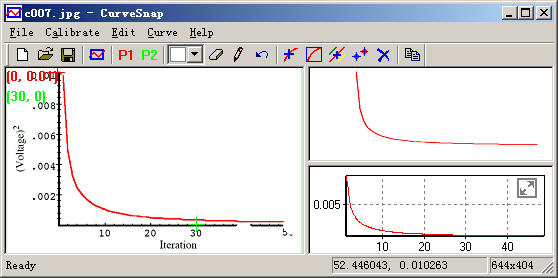
\includegraphics{./tut_files/00_curvesnap_wide.jpg}
\end{figure}
\tableofcontents

\newpage
This tutorial is really simple. You can ignore it and use the program directly.
\begin{figure}[ht!]
\section{Capture curve from screen - A first example}
  \center 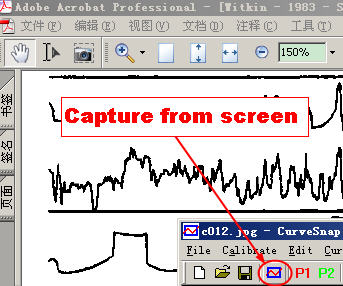
\includegraphics{./tut_files/01_capture.jpg}
\end{figure}

\begin{figure}[ht!]
  \center 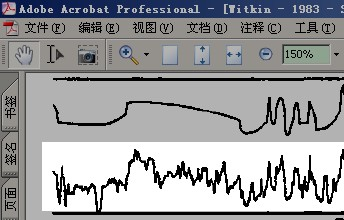
\includegraphics{./tut_files/02_capturing.jpg}
\end{figure}

\begin{figure}[ht!]
\section{Choose curve by connectivity}
  \center 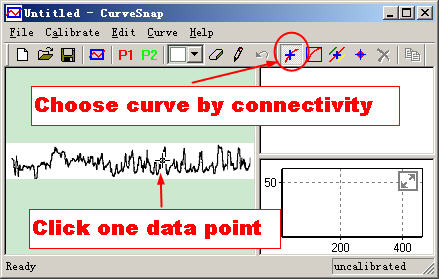
\includegraphics{./tut_files/03_choose_by_connectivity.jpg}
\end{figure}

\begin{figure}[ht!]
  \center 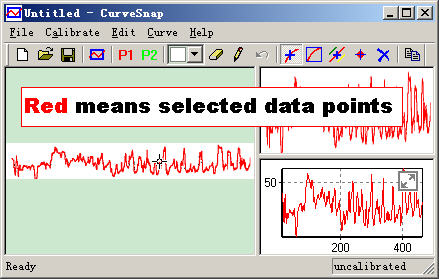
\includegraphics{./tut_files/04_chosen.jpg}

  Note that the curve is not calibrated yet. So the pixel coordinate is used.
\end{figure}

\begin{figure}[ht!]
\section{Copy the data}
  \center 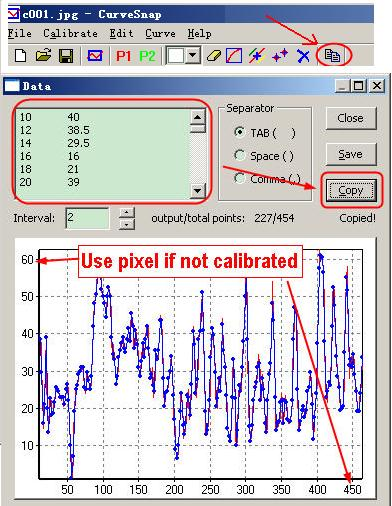
\includegraphics{./tut_files/05_copy_data.jpg}
  See the last section on V1.1 update
\end{figure}

\begin{figure}[ht!]
\section{Open existed image - A second example}
  \center 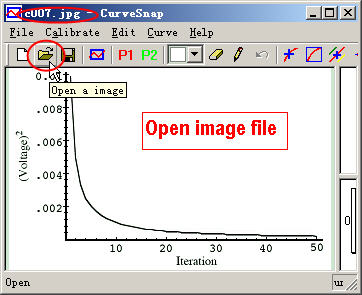
\includegraphics{./tut_files/06_open_image_file.jpg}
\end{figure}

\begin{figure}[ht!]
\section{Calibration}
  CurveSnap uses two points to calibrate the axis. The two points must not be close to each other horizontally or vertically. The picture below is actually from V1.0, while current version V1.1 is slightly different, with a magnified window to adjust the point.
  \center 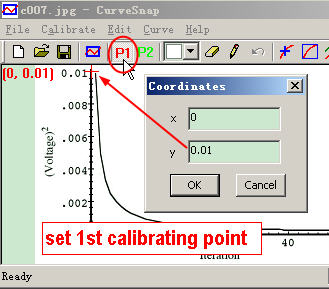
\includegraphics{./tut_files/07_1st_calibrating_point.jpg}
\end{figure}
\begin{figure}[ht!]
  \center 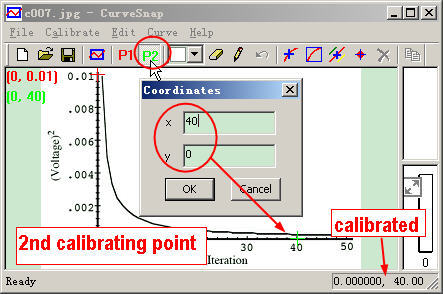
\includegraphics{./tut_files/08_2nd_calibrating_point.jpg}

  When both points are set, the status bar shows the calibrated coordinates under the cursor.
\end{figure}

\begin{figure}[ht!]
\section{Erase to make curve isolated}
  To use the tool \textbf{Choose by connectivity}, the data curve must not connected to axis, labels, grids, other curves, etc.
  \center 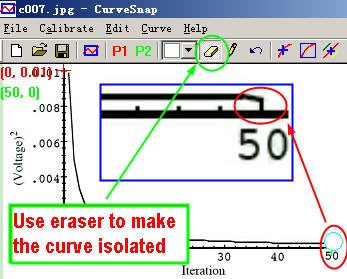
\includegraphics{./tut_files/09_eraser.jpg}
\end{figure}

\begin{figure}[ht!]
  \center 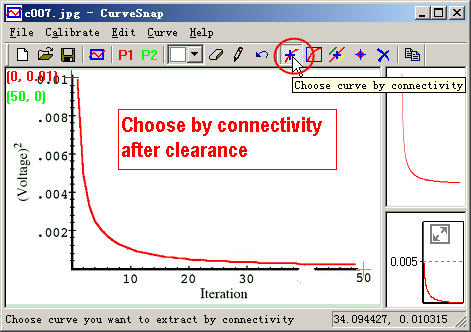
\includegraphics{./tut_files/10_choose_after_eraser.jpg}
\end{figure}

\begin{figure}[ht!]
\section{Choose data points by dragging a rectangle}
  \center 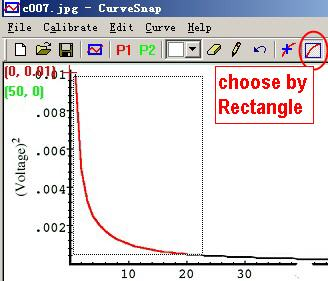
\includegraphics{./tut_files/11_choose_rect.jpg}
\end{figure}

\begin{figure}[ht!]
\section{Choose curve by its color}
  If the desired data curve is colored, then \textbf{Choose by Color} is recommended.
  \center 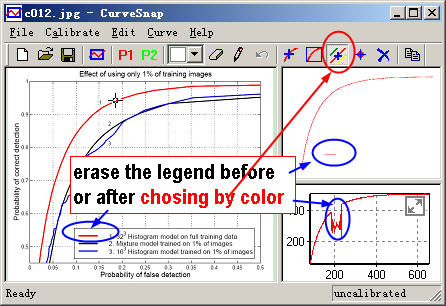
\includegraphics{./tut_files/12_choose_by_color.jpg}
\end{figure}

\begin{figure}[ht!]
  Note that the legend have the same color of curve, erase them.

  \centering{ 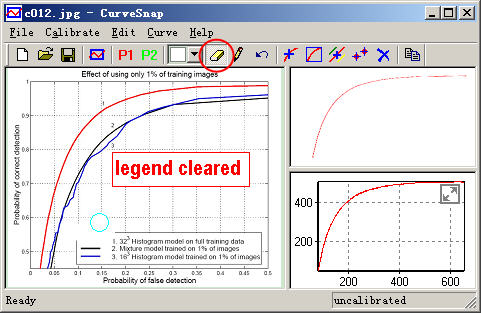
\includegraphics{./tut_files/13_legend_clear.jpg}}
\end{figure}

\begin{figure}[ht]
\section{Increase interval to make the extracted curve nicer}
  CurveSnap extracts data from pixel, which is digitized. The output data may look step-like if you export all of the data points. So it's recommended to increase the interval in this case.

  \centering{ 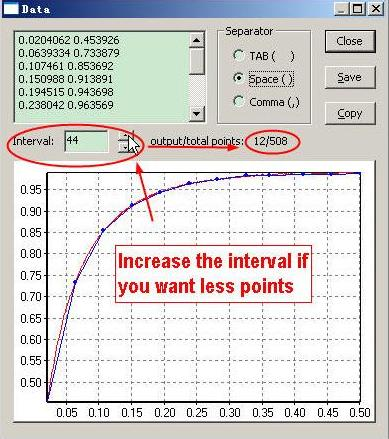
\includegraphics{./tut_files/14_interval.jpg}}
\end{figure}

\begin{figure}[ht]
  \centering{ 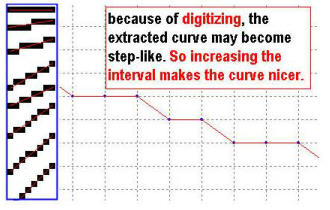
\includegraphics{./tut_files/15_digitizing.jpg}}
\end{figure}

\begin{figure}
\section{How does it work?}
  Average the foreground pixels in the vertical direction

  \centering 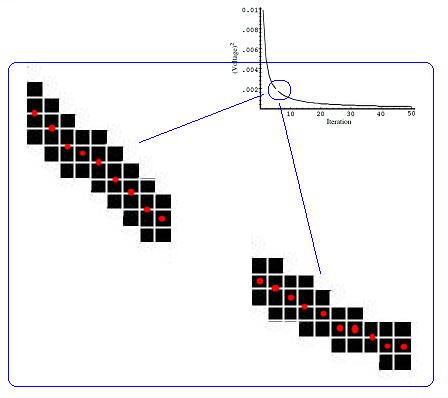
\includegraphics{./tut_files/16_how_does_it_work.jpg}
\end{figure}

\begin{figure}
\section{V1.1 Update: Output Control}
  The Linear Spaced settings of X Ticks is for users who want to customize the x coordinates, which can be interpolated from the original calibrated pixel data.
  \\[3ex]
  Output Precision. When \textbf{fixed is off}, the input represents the \textbf{decimal precision}. For example, pi is 3.14 under 3, 3.1416 under 5. Set to 0 to output all the digits(default).
  \\[3ex]
  When \textbf{fixed is on}, the input represents the \textbf{number of digits following the decimal point}, and pi is 3 under 0, 3.14 under 2. Another example, setting fixed on and input 0 results in integer outputs.
  \\[3ex]
  For c++ programmers, the above is straightforward, just about std::setprecision and std::fixed.

  \centering 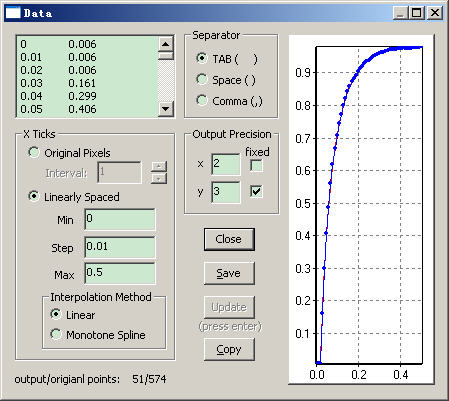
\includegraphics{./tut_files/21_v1p1_update_data_dialog.jpg}
\end{figure}
\end{document}
